\chapter{WAN Based DC Energy Simulations for Internet Services}
\label{chp:traffic}

\section{Chapter Abstract}
    Data centers (DCs) are a critical component of modern day economies and social lives of people all around the world. In many aspects society’s dependency on internet services enabled by DCs is still increasing; the COVID-19 stay in place orders are a current example of unprecedented growth rates for many internet services. With the increasing dependency on DCs, there is a concern about their environmental impacts. Reasoning about the environmental footprint of these globally spanning infrastructure systems requires new approaches for modeling energy use of facilities within these systems. This work demonstrates such as model with a prototype of a top down software module that simulates the traffic profile for a globally distributed internet service. Using Wikipedia as the exemplary internet service, the developed simulator's results are used to reset the IT loads in EnergyPlus to quantify the power demand required to operate all the buildings within the network of Wikipedia DCs.   
    


\section{Introduction}

    DCs are ubiquitous in today’s society. Consumers of DC enabled web services expect high availability of their functionality and access to their data on a continual basis. These expectations are met with software architectures that provide strongly consistent views of the data regardless of location and in the presence of physical systems failures. In terms of specific failure modes, network failures can be the most catastrophic. For example, an outage of a network link connected to a DC can lead to all it's physical resources to become inaccessible from the outside. With these expectations, the dependencies between internet DCs and their communications network during failures is clearly apparent.
    
    The utility systems (such as mechanical cooling and power distribution) and the network connections of a DC are not only coupled in failure scenarios described above, but they are in lock-step with each other during normal operations too. This coupling of network and building systems is easy to reason about as internet DCs don’t generate workloads hermetically. The workload demands for DCs come from remote consumers (user facing traffic) and other adjacent DCs (back-end traffic). Both forms of incoming traffic instantiate computational and storage processes on the IT hardware, which in turn are powered and cooled by district scale distribution plants.
    
    In the current generation of DCs, the building utility systems demand less than 10\% of the total energy delivered to the site \cite{Shehabi16}. The balance of the power of these new DCs is consumed by the information technology (IT) equipment. With this disproportionate allocation of energy, it is clear that the total energy use in DCs is more sensitive to IT loads than the facilities systems. Yet the building systems still receive the most attention in the design and facilities operations phases of the buildings. Others have pointed out gaps in the current DC building energy modeling practices as-well \cite{Beatty15}. 
    
    To provide an intuition of DC networks, Figure~\ref{net_diag} shows a generalized depiction of their topology. At the top, the internet service provider (ISP) networks are shown as clouds because the physical paths of these systems are managed by the global ISPs and are typically out of the control of DC operators. DC operators depend on the ISP's physical infrastructure for connecting their geographically remote facilities with private wide area networks (WAN). The pink links indicate these WAN connections that traverse over ISP networks. The magenta links connect global WAN's to DC metropolitan areas, which typically are responsible for the last miles of network distribution. Within the metropolitan area, there maybe one or more DC sites, only two are shown for clarity in the figure. 
    
    \begin{figure}[h]
\centering
    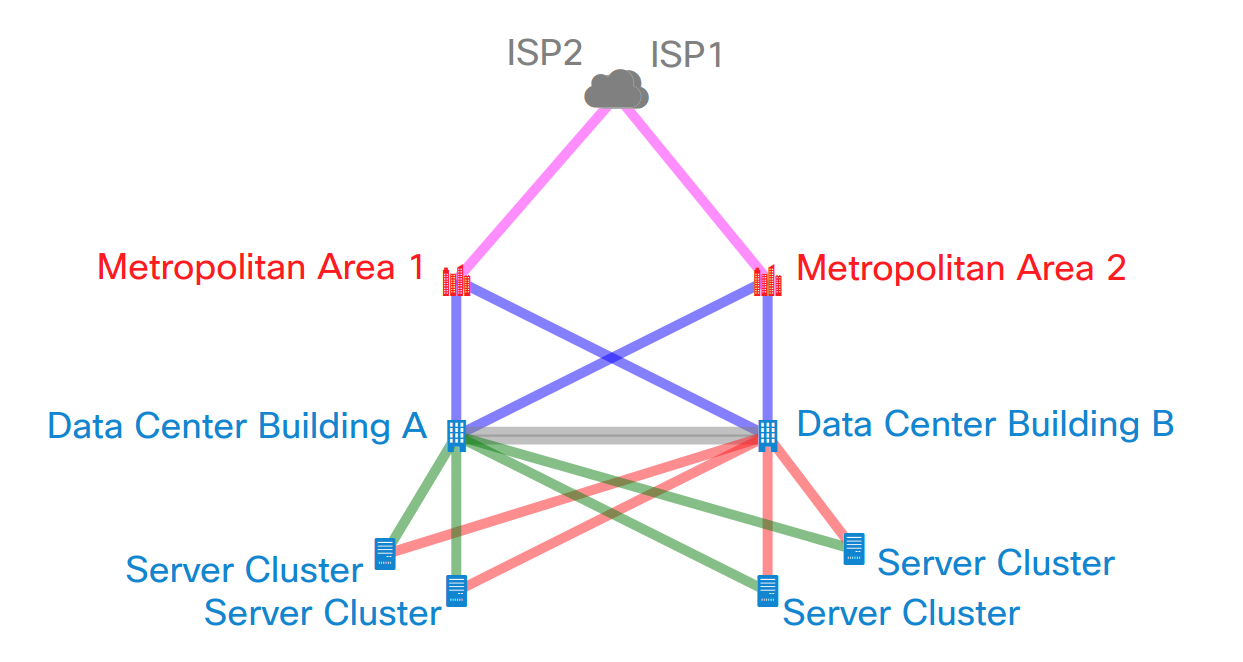
\includegraphics[scale=0.2]{traffic_profile/images/net_diag.png}
    \caption[Network Diagram]{Generic Data Center Network Topology.}
\label{net_diag}
\end{figure}

    
    From a business perspective, the data center construction spending is estimated to reach \$89 billion by 2027. The estimate nearly doubles the spend seen in 2018 \cite{dcmarket19}. At the core, the demands for DCs is driven by the expected consumer traffic to its services. With this much value at stake, capital and operational decisions must be based on robust system level models that couple IT traffic and DC designs.
    
    The business and operational dependencies of network traffic to building loads as discussed above motivate this work. The work couples IT demands with building level resource utilization by first developing a simulator to demonstrate a method for geographically correlating five DCs with the incoming visits from a global user base using a minimum cost function. The resulting correlations are further extended to provide a forecast of the traffic. The generated traffic profile from the network simulator is interactively coupled used with EnergyPlus to reset the IT load at each time-step. 
    
    The contribution of this research is two-fold. First, it demonstrates a way to reason about network traffic profiles by developing a network simulator based on abstract usage data for a global internet service. Second, it validates that DC operators and designers can model future demands of building infrastructure systems and perform scenario models based the predicative characteristics of network traffic. 
    
\section{Literature Reviews}
    EnergyPlus, the US Department of Energy’s building energy modeling software has supported DC modeling since release 8.3 [4]. The EnergyPlus modeling capability allows for IT equipment load schedules to be explicitly modeled in it. Today, EnergyPlus comes with three example DC models, in the form EnergyPlus Input Files (IDF). These IDFs provide a template that energy analysts can extend and augment to represent their specific DC designs. These default templates are hermetic and lack coordination with dynamic workloads that are prevalent in data centers. Dynamic behaviors of various internet applications inside DCs is presented by Harhol-Balter in \cite{harchol13}. However, there are proven techniques to integrate the dynamic behavior of DCs in EnergyPlus with supplemental software applications that allow for an interactive feedback loop with it. Building Control Virtual Test Bed (BCVTB) is one such application \cite{EnergyPlus8.3}. 
    
    Wei demonstrates the use of BCVBT for modeling a mixed used facility that has a DC collocated with occupied spaces in \cite{wei17}. Zhang demonstrated the use of BCVTB for the control of an educational building \cite{zhang19}. Zhang published their Python code base to allow others to replicate their work. Functionally, BCVTB creates an interactive process loop with EnergyPlus allowing the Python program to be aware of EnergyPlus simulations at every simulation time step. Figure~\ref{agent_bem} illustrates the interactive loop between EnergyPlus and a Python software agent that is implemented in the developed module of this work. In the next paragraph, background about WAN from an internet service perspective is provided. 
    
    \begin{figure}[h]
\centering
    
\includegraphics[scale=0.15]{traffic_profile/images/agent_bem.png}
    \caption[Software Agent and BEM Interaction]{General process flow between EnergyPlus and internet traffic simulation.  .}
\label{agent_bem}
\end{figure}
    
    WANs serve as the backbone for many internet applications that operate across regionally distributed DCs. The traffic on WAN links are segregated into three classes; interactive, large file transfers, and background. LinkedIn’s experience with these three classes of traffic is document well by Zhuang \cite{zhuang15}. Interactive traffic consists of blocking operations, where the sequential byte level transactions are required to keep things proceeding. Large file transfers entail transmission of requested resources by an explicit deadline. An example of a deadline based application is a data transfer required for a status report that must be generated a particular time. Background traffic are workloads that are ok with opportunistic network availability and are resilient to any idempotent side effects in case the traffic gets preempted due to higher priority traffic. These three classes of traffic can either be user facing or back-end. Microsoft and Google have both published their experiences in designing and operating these massive global networks \cite{hong13, sushant13}.  

\section{Methodology} 
    In this section the methods for characterising network traffic and correlating it with DC workloads is described. First, three step-wise methods that support the development of a network traffic simulator are presented. Namely these methods are:
    
    \begin{enumerate}
        \item The selection of a service level data-set that can characterize a global scale internet platform with a dispersed user base and geographically distributed data centers. 
        \item Abstraction of the service level information to map its network traffic to one of the data centers in the network, 
        % \item The correlation of the data center level traffic to the power demands from operating the service in a data center. 
        \item A method to scale historical service demands into projections of future workloads for the DCs.
    \end{enumerate} 
    
    \subsection{Selection criteria for selecting the global service to model}

    Below are the key criteria that was set for a representative global scale service:
    \begin{enumerate}
        \item High resolution usage data publicly available.
        \item Non-Proprietary and acceptable for publications. 
        \item A service with global user base.
        \item Representative of a distributed service with geographically dispersed data centers.
        \item Publicly available data on physical infrastructure.
    \end{enumerate}
    
    For the purposes of this research as a prototype model, Wikipedia.com was found to meet the entire list of the set criteria. First, a high resolution usage data-set was publicly available through a Kaggle.com forecasting competition \cite{kaggle17}. The second criteria was satisfied by Wikipedia's source code and infrastructure design being free and open under MediaWiki copyright terms \cite{wiki_media}. The obtained Wikipedia data-set represented seven natural languages. With naive association of the natural languages to the countries that they are the official national language, the data-set met the second criteria for a global user base. For compliance with the fifth criteria, Wikipedia's engineering site validated it's geographically dispersed DC infrastructure \cite{wiki_locs}. Given the free and open copy right terms, several key infrastructure attributes for Wikipedia data centers are readily available on the internet, meeting the fifth criteria.
    
\subsection{Service Level Abstraction}
    
    Meta information and statistical attributes of the Kaggle data-set has been used to develop the network simulator presented in this work. The data-set included traffic in counts of daily visits to 145,063 Wikipedia Pages for 803 days from July 2015 through September 2017. The data is partitioned differently for training and testing the predictive models. The training set is inclusive of traffic from July 2015 to December 2016. The remaining data is used to test the accuracy of the models. 
    
    All pages are segregated into 7 different languages. Namely the languages are English, Japanese, German, French, Chinese, Russian, and Spanish. Each page's natural language is extracted from the meta information embedded in the URL strings that are included with the original data-set. As an example, consider the following URL string below.
    
    \begin{verbatim}
        1918_flu_pandemic_en.wikipedia.org_desktop_all-agents
    \end{verbatim} 
    
    The regular expression pattern search command re.search('[a-z][a-z].wikipedia.org',page) is used to extract the language meta data. For the example URL, regular expression search returned 'en' for English.  For each language, the mean volume of visits per language is shown in \ref{mean} and the 95th quantile is shown in \ref{95thquantile}.  
    
    \begin{figure}[!htn]
  \subfloat[Mean Value of Page Views]
  {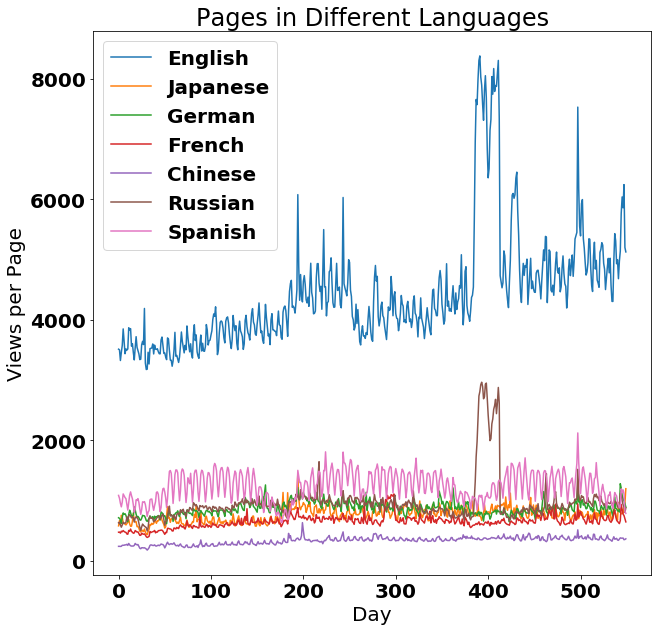
\includegraphics[width=0.5\textwidth]{traffic_profile/images/mean.png}\label{mean}}
  \hfill
  \subfloat[$95^{th}$ Quantile Value of Page Views] 
  {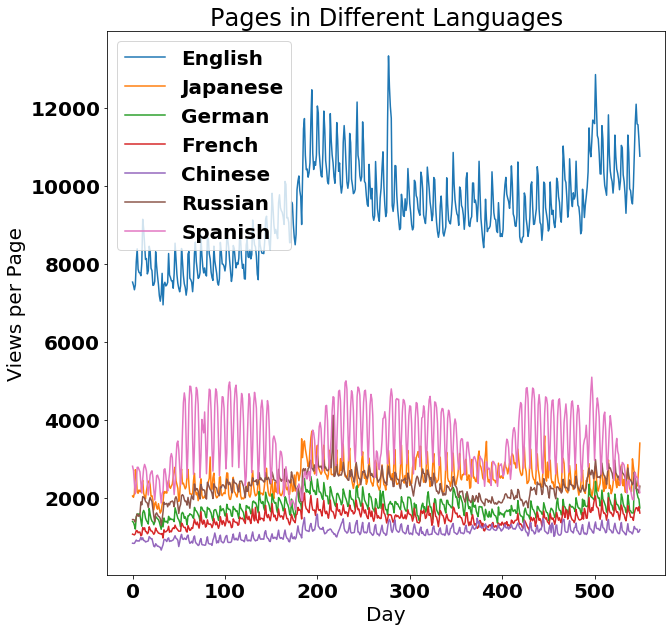
\includegraphics[width=0.5\textwidth]{traffic_profile/images/quantile95_use.png}\label{95thquantile}}
  \caption[Page Views by Language]{Pages Views for Each Language}
\end{figure}
        
    The curves in Figure~\ref{mean} and Figure~\ref{95thquantile} are indicative of the distribution of daily visits for each of the seven languages found in the data-set.  For example, the 95th quantile represents pages that had more visits than 95\% of the pages in the particular language on a given day. In the figure, the y-axis indicates the count of visits on the corresponding day noted on the x-axis. While the average curves indicate the average number visits to pages in the respective language on the corresponding day. Both of these curves can be used in the design phase of the DC buildings, with the 95 quantile determining the capacity and the average values supporting operational models. In this article, the average value is used as the indicator of the operational network model. 
    
    \definecolor{chinese}{rgb}{0, 1, 0} %chinese 
\definecolor{english}{rgb}{0, 0, 1}%english 
\definecolor{french}{rgb}{.8, 0, 0}%french 
\definecolor{german}{rgb}{.5, .5, .5}%german 
\definecolor{japanese}{rgb}{0, 0, .5}%japanese 
\definecolor{russian}{rgb}{0, .5, 0}%russian 
\definecolor{spanish}{rgb}{.20, .92, .85}%spanish 


\begin{figure}[h]
\centering

        \begin{tikzpicture}
        \begin{scope}[xshift=1.5cm]
            \node[anchor=south west,inner sep=0] (image) at (0,0)
            {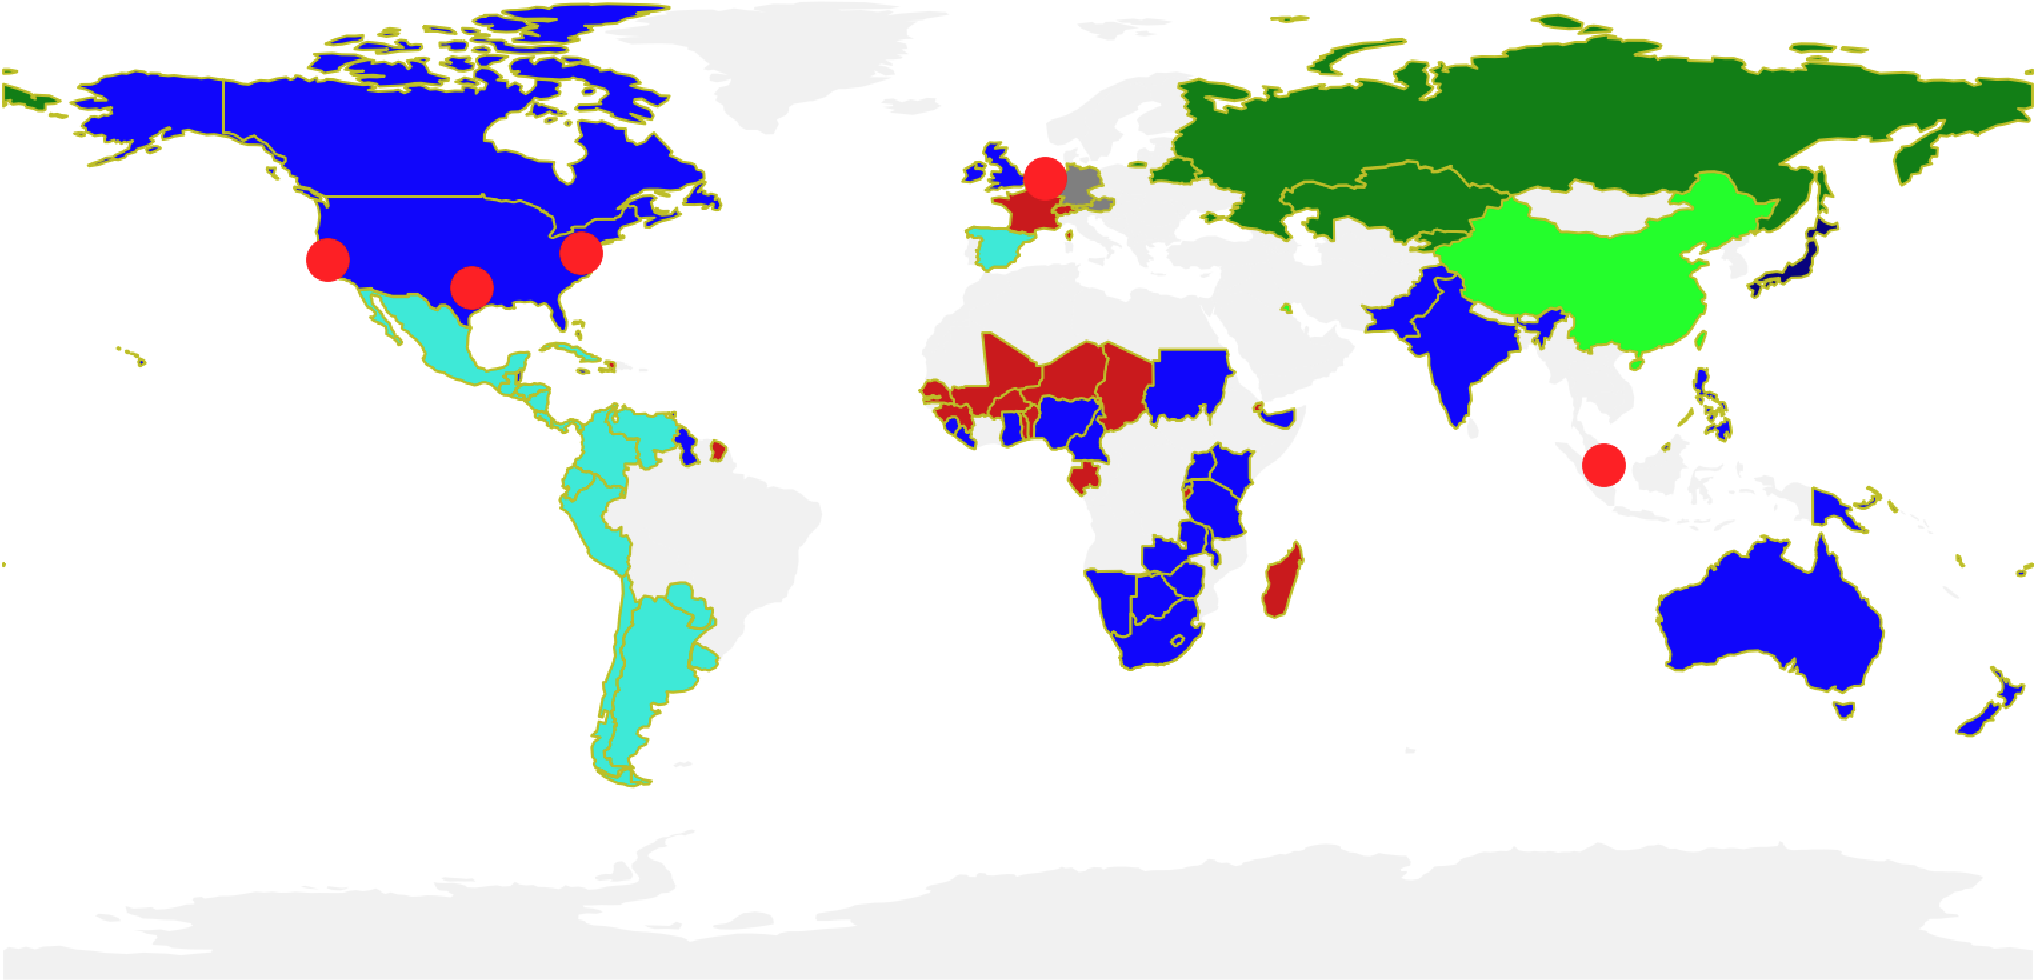
\includegraphics[width=1\textwidth]{embodied_cost_model/images/worldmap_4.png}};
        \end{scope}
        
        \begin{scope}[xshift=1.0cm]
            \node [anchor=center] (chinese) at (2,-.6) {\small{Chinese}};
            \filldraw[outer color=chinese, inner color=chinese] (1.8,-.4) rectangle (2.2,0); % chinese
            
            \node [anchor=center] (english) at (4,-.6) {\small{English}};
            \filldraw[outer color=english, inner color=english] (3.8,-.4) rectangle (4.2,0); % english
            
            \node [anchor=center] (french) at (6,-.6) {\small{French}};
            \filldraw[outer color=french, inner color=french] (5.8,-.4) rectangle (6.2,0); % french
            
            \node [anchor=center] (german) at (8,-.6) {\small{German}};
            \filldraw[outer color=german, inner color=german] (7.8,-.4) rectangle (8.2,0); % german
            
            \node [anchor=center] (japanese) at (10,-.6) {\small{Japanese}};
            \filldraw[outer color=japanese, inner color=japanese] (9.8,-.4) rectangle (10.2,0); % japanese
            
            \node [anchor=center] (russian) at (12,-.6) {\small{Russian}};
            \filldraw[outer color=russian, inner color=russian] (11.8,-.4) rectangle (12.2,0); % russian
            
            \node [anchor=center] (spanish) at (14,-.6) {\small{Spanish}};
            \filldraw[outer color=spanish, inner color=spanish] (13.8,-.4) rectangle (14.2,0); % spanish
            
            \node [anchor=center] (dc_location) at (9,-1.1) {\small{Data Center Locations}};
            \filldraw[red] (7,-1.1) circle (4pt); 
            
            \end{scope}
            
        \end{tikzpicture}

\caption[Source country of language and DC locations]{Source country of language and DC locations map.}
\label{image:world_language_map_wan}
\end{figure}
    
    After segregation of the pages by language and dropping pages without language indicators, the languages are mapped to countries in which they are the official language. Figure~\ref{image:world_language_map_wan} shows the mapping of languages to their respective countries by color groups; English (blue), Japanese (navy blue), German (gray), French (red), Chinese (light green), Russian (forest green), and Spanish (cyan). Red markers indicate the locations of Wikipedia DCs from around the world as listed in Table~\ref{language_to_dc}.
    
    
\begin{table}[h!]
    \begin{center}
    \scalebox{0.8}{
    \pgfplotstabletypeset[
        col sep=comma,
        string type,
        columns/DC/.style={column name=DC, column type={|l}},
        columns/en/.style={column name=English, column type={|c}},
        columns/ja/.style={column name=Japanese, column type={|c}},
        columns/de/.style={column name=German, column type={|c}},
        columns/fr/.style={column name=French, column type={|c}},
        columns/zh/.style={column name=Chinese, column type={|c}},
        columns/ru/.style={column name=French, column type={|c}},
        columns/es/.style={column name=Spanish, column type={|c}},
        columns/total/.style={column name=Total, column type={|c|}},
        every head row/.style={before row=\hline,after row=\hline},
        every last row/.style={after row=\hline},
        ]{traffic_profile/content/data/Language_to_DC.csv}}
    \end{center}
    \caption[Languages to Ingress Sites]{Languages to Ingress Sites}
    \label{language_to_dc}
\end{table}


    
    Throughout this research these Wikipedia DCs are used to the model the network based on publicly available information. Several additional assumptions are made in regard to the attributes of the system that are not in the public domain. Furthermore, some of the system complexity is reduced for brevity. For example, the traffic generating in a particular country is allocated with their closest ingress points as listed in Table~\ref{language_to_dc} by using a minimum distance function between the respective geographical codes. 
    
    The specific step-wise approach of mapping languages to the respective DC is shown in Table~\ref{traffic_allocation_steps}. Following these steps, Figure~\ref{land_dc_sankey_wan} shows that English is the most dominant language, with its traces appearing at all of Wikipedia's ingress sites while originating in 49 countries.  
    
    \begin{table}[h!]
    \begin{center}
    \scalebox{0.8}{
    \pgfplotstabletypeset[
        col sep=comma,
        string type,
        columns/Steps/.style={column name=Steps, column type={l}},
        columns/Description/.style={column name=Description, column type={l}},
        every head row/.style={before row=\hline,after row=\hline},
        every last row/.style={after row=\hline},
        ]{traffic_profile/content/data/traffic_allocation_steps.csv}}
    \end{center}
    \caption[Method for Traffic Allocation to each ingress site ]{Method for Traffic Allocation to each ingress site }
    \label{traffic_allocation_steps}
\end{table}
    
     \begin{figure}[h!]\centering
    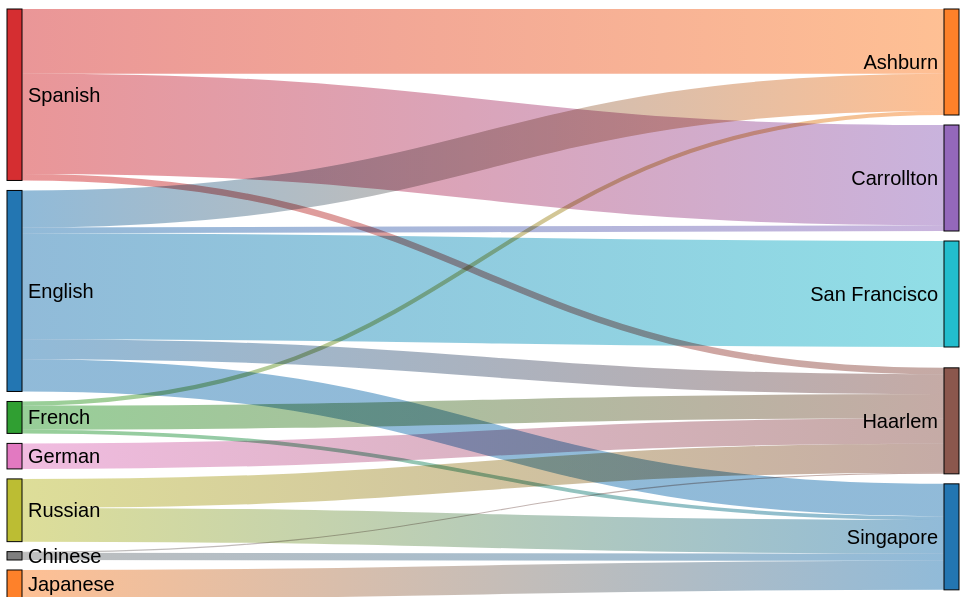
\includegraphics[scale=0.4]{embodied_cost_model/images/sankey_dc_03.png}
    \caption[Language to Data Center Site Sankey Diagram]{Language to data center flows. The thickness of the links at each data center site indicate the relative portion of traffic that the respective language demands at the data center.}
    \label{land_dc_sankey_wan}
    \end{figure}
    
    \subsection{Scaling service demands into the future}
    
    In this section, the Wikipedia traffic profiles are used to forecast future demands. Note that the traffic data is slightly modified to represent digital bits (instead of visit counts) in order to demonstrate another useful insight that network traffic inherently provides. The objective here is to determine the future service demands that drive workloads at each DC. To obtain the digital payload of the pages, their contents are converted to byte (8-bits) size representation. The bit size distribution of Wikipedia articles was not readily available in the public domain so an estimation method was developed for this work. First, several resources were consulted to determine the page size \cite{wiki_stats, xtools}. The resulting page sizes for each of the seven languages studied in this article are noted in Table~\ref{language_to_page_size}. 
    
    \begin{table}[h!]
    \begin{center}
    \scalebox{0.8}{
    \pgfplotstabletypeset[
        col sep=comma,
        string type,
        every head row/.style={before row=\hline,after row=\hline},
        every last row/.style={after row=\hline},
        ]{traffic_profile/content/data/language_to_page_size.csv}}
    \end{center}
    \caption[Language to Page Size Classification]{Language to Page Size Classification}
    \label{language_to_page_size}
\end{table}    
    
    With the bit wise representation from Table~\ref{language_to_page_size}, the time series of the traffic can be analyzed to make future predictions. The time series ($t$) dependencies of a variable $X$ can generally be decomposed in trending ($T$), seasonal ($S$), and random ($R$) components, as shown in Equation \ref{eq: ts_forecasts} \cite{zhuang15}. \begin{equation} X_t = T_t + S_t + R_t \label{eq: ts_forecasts} \end{equation} More specifically $T$ exists when there is a gradual shift across time, $S$ indicates cyclic patterns, and $R$ accounts for randomness.   
    
    In the next few paragraphs two forecasting methods that decompose the time-series into these three components are presented and their implementations along with their results are discussed. Namely these methods are:
    \begin{enumerate}
        \item The Auto Regressive Integrated Moving Average \textit{(ARIMA)}, an open source statistical forecasting software suite \cite{arima_py}.
        \item As an alternate to ARIMA, Generalized Additive Model (GAM) is a proven method to forecast internet traffic. Specifically Facebook's \textit{Prophet} implementation of GAM is implemented \cite{fbprophet}.
    \end{enumerate}
    
    \emph{ARIMA Model}: First, time-series analysis is performed using the Auto Regressive Integrated Moving Average (ARIMA) model. The auto regression component leverages the dependencies between an observation and some lagged time step. The integration component differentiates the raw observations from preceding time steps to make the series stationary. The moving average component quantifies the dependency between observations and residual errors with a moving average model applied to lagged observations. Each of the three components are specified as a model input parameter in the form ARIMA(p, d, q). The parameter p indicates the lag order, d indicates the degree of difference (i.e. subtract the previous value from the current value), and q indicates the size of the moving window (the moving average) \cite{arima_def}. 
    
    The ARIMA model has been used effectively in previous literature to forecast 21 days of network traffic with 42 days of past trends \cite{zhuang15}. This research extends the forecast out to 9 months using 18 months of past trends. The resulting output from ARIMA are shown in Figure~\ref{arima}. Figure~\ref{arima}’s legend indicates the use of combination of ARIMA(2,1,2) and ARIMA(1,2,4) as parametric arguments to the ARIMA module. The lighter curves indicate ARIMA's predicated values and the darker curves indicate real data that was held back as the 'testing partition' described earlier. These results indicate that ARIMA can produce reasonable forecasts over a time horizon that may be conducive for DC design and operational decisions. 
    
    \begin{figure}[h]
\centering
    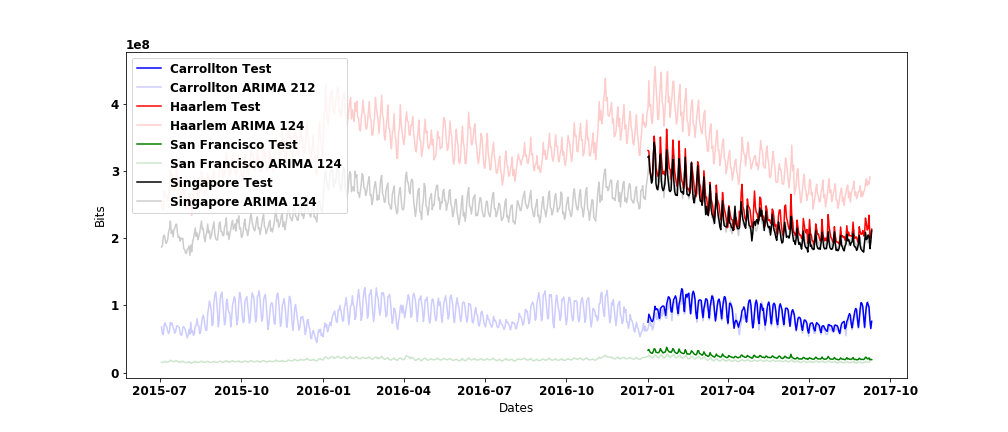
\includegraphics[scale=0.4]{traffic_profile/images/_arima.png}
    \caption[Network Diagram]{ARIMA Models: Historical trends and future projections.}
\label{arima}
\end{figure}
    
    \emph{Generalized Additive Model}: Next, a variant of the generalized additive model (GAM) was simulated with the same bit wise time series as used in the ARIMA simulations. The model is explained in great detail by Taylor in \cite{fbprophet}. The GAM model variant, Prophet, has a decomposable time series formulation similar to the time series dependence indicated in Equation~\ref{eq: ts_forecasts}. However, Prophet is supplemented with a term that accounts for holidays that occur at idiosyncratic  intervals. 
    
    Furthermore, Prophet has a novel concept that deals with trends in forecast uncertainty, in that it uses a Laplace transform to randomly distribute future change points in the trend based on past data \cite{fbprophet}. This can be seen by how closely the forecasts (blue lines) track the historical data (black dots) and the actual forecast based on the test data (magenta lines) in Figures~\ref{DFW}, \ref{AMS}, \ref{SFO}, \ref{SIN}. The change point parameter is set to $0.3$ and the yearly seasonality parameter is set to $True$ for these simulations. The forecast extends beyond the test data range which shows that the cone of uncertainty increases as the forecast is extended out further, indicated by the light blue curves. 
    
    \begin{figure}[!htn]
  \subfloat[Carrollton (DFW)]
      {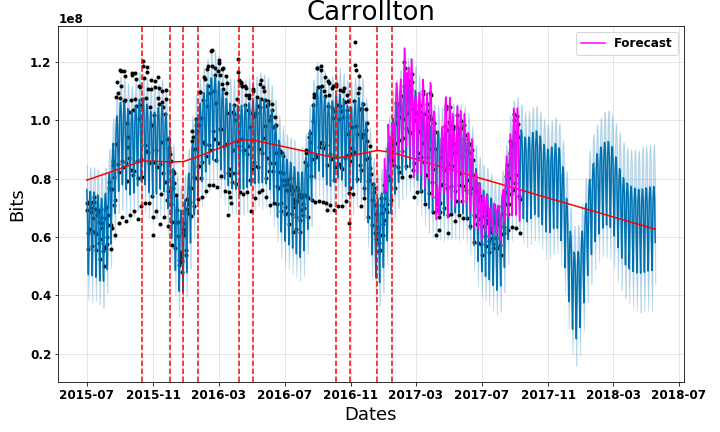
\includegraphics[width=0.5\textwidth]{traffic_profile/images/Carrollton_prophet.png}
      \label{DFW}}
  \hfill
  \subfloat[Haarlem (AMS)]
      {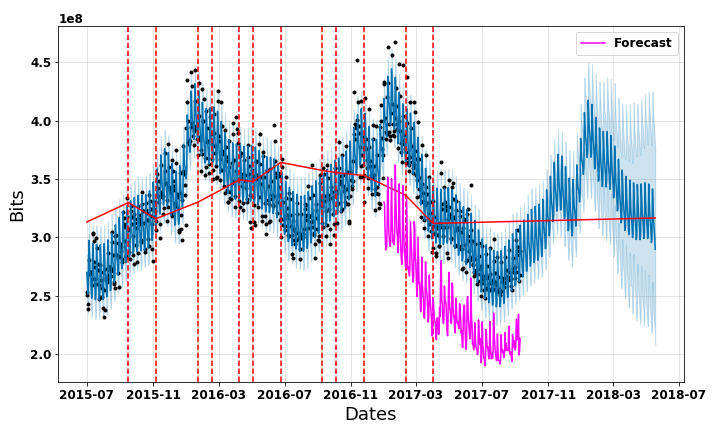
\includegraphics[width=0.5\textwidth]{traffic_profile/images/Haarlem_prophet.png}
      \label{AMS}}
  \hfill
  \subfloat[San Francisco (SFO)]
      {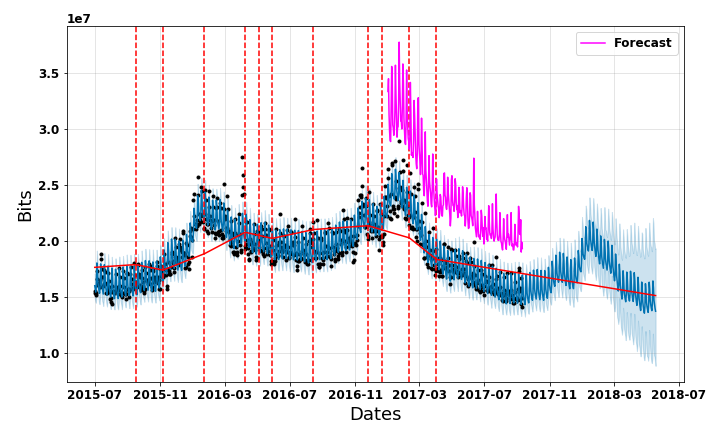
\includegraphics[width=0.5\textwidth]{traffic_profile/images/SanFrancisco_prophet.png}
      \label{SFO}}
  \hfill
  \subfloat[Singapore (SIN)]
      {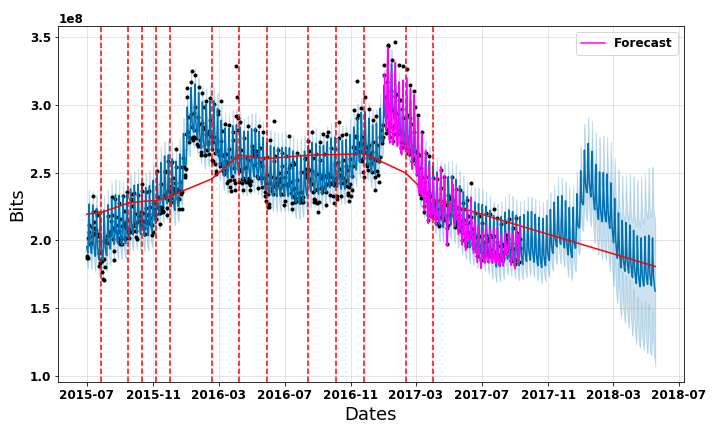
\includegraphics[width=0.5\textwidth]{traffic_profile/images/Singapore_prophet.png}
      \label{SIN}}
  \hfill
  \caption[Prophet Curves]{Prophet Historical Trends and Traffic Forecast}
\end{figure}
    % Provide a compartive table for MAPE of Arima and Prophet
    
    Table~\ref{mape} provides a comparison of the mean absolute error (MAPE) for four DC sites. The difference in error rates varies by a factor of 1.72 (for SIN) and over 52 (for SFO). Overall, in comparison it is shown that the Prophet model is superior to the ARIMA model in terms of accuracy of its predications. 
    \begin{table}[h!]
    \begin{center}
    \scalebox{0.8}{
    \pgfplotstabletypeset[
        col sep=comma,
        string type,
        every head row/.style={before row=\hline,after row=\hline},
        every last row/.style={after row=\hline},
        ]{traffic_profile/content/data/mape.csv}}
    \end{center}
    \caption[MAPE for ARIMA and Prophet Models]{Mean Absolute Percentage Error}
    \label{mape}
\end{table}
    
\section {Results}

    In this section the results from using the traffic coefficients is presented. Following the steps listed in Table~\ref{traffic_allocation_steps} yields the curves indicated in Figure \ref{ingress_hitrate_95_links}. Each curve in the figure is inclusive of all the languages that are routed to the respective data cent. 
    
    To reason about these curves, recollect the distribution of the languages at each DC from Table~\ref{language_to_dc}. For example, the curve for San Francisco (SFO) in Figure~\ref{ingress_hitrate_95_links} is nearly 100 times smaller than the curve for the Haarlem (AMS) site. This is due to only four countries being routed to San Francisco (the US is routed to Carrolton by the method used), whereas Haarlem has traffic routed from 38 countries. This naive approach evenly apportions the total count of the language's page visits equally to all countries in which it is the national language, regardless factors such as population or size.   
    
    Figure~\ref{cpu_site} shows the resulting CPU power profile for the English languages pages when using their traffic coefficients in EnergyPlus simulations at four DCs. The coefficients are based on the average page view values from Figure~\ref{mean}. The details of the EnergyPlus configuration are provided by Kumar in \cite{kumar20, kumar20b}. Since the English language is the dominate language at the San Francisco site nearly all of the CPU resources at the site are dedicated to it. The constant load profile for San Francisco can be attributed to the corresponding flat curve shown in Figure~\ref{ingress_hitrate_95_links}. 
    
    \begin{figure}[h]
\centering
    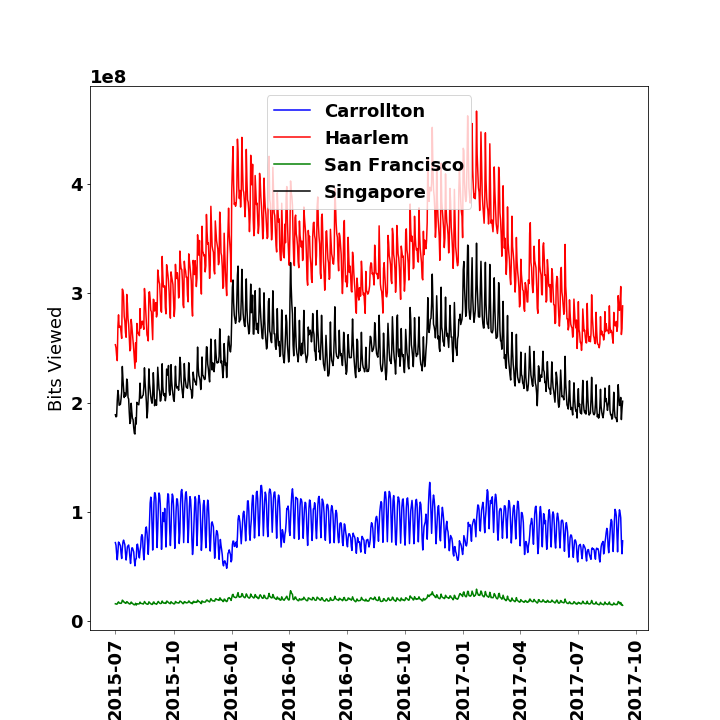
\includegraphics[scale=0.35]{traffic_profile/images/ingress_hitrate_95_links.png}
    \caption[Total Traffic to Each Site after mapping]{Total Traffic to Each Site after mapping.}
\label{ingress_hitrate_95_links}
\end{figure}
    
    \begin{figure}[h]
\centering
    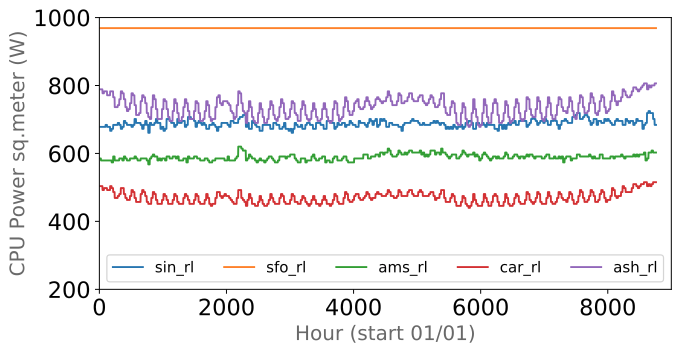
\includegraphics[scale=0.4]{traffic_profile/images/site_profile.png}
    \caption[CPU-Site Profile]{Plot of EnergyPlus CPU Profiles with the Network Coefficients .}
\label{cpu_site}
\end{figure}
    
\section{Conclusion}
    The methods used in this chapter are indicative of a process that requires DC designers to first understand functional requirements of their distributed software systems. Once the underlying services are understood they need to be characterized by their geographical boundaries as done in the Service Level Abstraction section. In this study, languages are analogous to traditional internet services and the count of page views are used as the sole usage metric. Once the service boundaries are established, correlations between the physical resource dimensions can be configured as done in the EnergyPlus model discussed in the Results section. Specifically in this work, WANs were correlated to power demands at the DCs. The conversion of a network demands to power translates intrinsic software service attributes into a unit of measure that is more intuitive for building energy analysts and DC building designers. The presented service abstraction method only serves as proof of concept, service specific models are required to make this strategy effective. An example of the service specific model is shown in \cite{zhuang15}.

    DC designers can use network profiles to implement energy models which assess their design choices at a single site or global level. At a single site level the building system components can be matched better with real demands. For example, if a service’s demand is at a low point on cool winter night, the cooling plant’s operating parameters just need to meet that low utilization point as opposed meeting the peak IT loads on the summer design day condition. This fine grained coupling may potentially lower the capital costs of the equipment at design time (if there is high confidence that peak traffic will not occur on the summer design day). In addition to capital savings, the network aware building systems can also supplement continuous load balancing strategies that optimize the total system by over subscribing the IT loads. Over subscription is feasible during part load conditions when the headroom in the electrical infrastructure can be exploited. Future work should look at a dynamic feedback loops to optimize network load balancing strategies and building controls. 